\documentclass{standalone}

\usepackage{tikz}
\usetikzlibrary{backgrounds, positioning, shapes.symbols}
\usepackage{helvet}
\renewcommand*{\rmdefault}{\sfdefault}

\begin{document}
\begin{tikzpicture}
  [
    font=\footnotesize,
    faraday/.style={minimum size=3cm, draw, dashed},
    duplexer/.style={draw,fill=white},
  ]

  \node[label=above:avra] (avra)
    {
\includegraphics[width=1.2cm]{server}};
  \node[right=0.5cm of avra, label=above:USRP N310] (n310gnb)
    {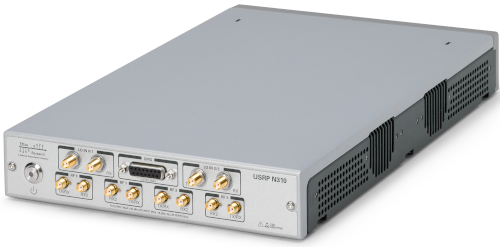
\includegraphics[width=1.2cm]{n310}} edge (avra);
  \node[right=.2cm of n310gnb, duplexer] (b78o) {n78} edge (n310gnb);
  \node[right=0.5cm of b78o] (ant1)
    {
\includegraphics[width=0.3cm]{antenna}} edge (b78o);
  \node[left=0.5cm of avra] (oc)
    {
\includegraphics[width=1.2cm]{openshift}} edge (avra);

  \node[right=7cm of n310gnb, label=above:caracal] (caracal)
    {
\includegraphics[width=1.2cm]{server}};
  \node[left=0.5cm of caracal, label=above:USRP N310] (n310ue)
    {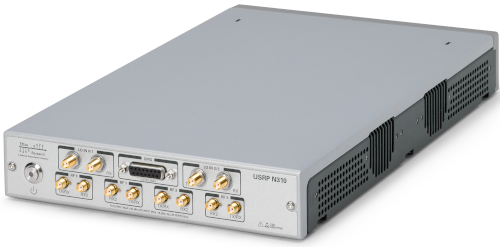
\includegraphics[width=1.2cm]{n310}} edge (caracal);
  \node[left=.2cm of n310ue, duplexer] (b78a) {n78} edge (n310ue);
  \node[left=0.5cm of b78a] (ant2)
    {
\includegraphics[width=0.3cm]{antenna}} edge (b78a);


\end{tikzpicture}
\end{document}
